\section{Patterns 2 - GoF Observer}

\subsection{Fokuspunkter}

\begin{itemize}
	\item Redegør for, hvad et Software Design Pattern er.
	\item Redegør for opbygningen af GoF Observer.
	\item Sammenlign de forskellige varianter, af GoF Observer - hvilken vil du anvende hvornår?
	\item Redegør for, hvordan anvendelsen af GoF Observer fremmer godt software design.
	\item Redegør for fordele og ulemper ved anvendelsen af GoF Observer.
	\item Redegør for, hvilke(t) SOLID-princip(per) du mener anvendelsen af GoF Observer undersøtter.
\end{itemize}

\subsection{Hvad er et Software pattern?}

\derp

\subsection{Redegør for opbygningen af GoF Observer}
Opbygningen kan ses på figur~\ref{fig:observer_classdiagram}, \pageref{fig:observer_classdiagram}, som viser et klassediagram for opbygning af dette pattern.

\begin{figure}[h]
	\centering
	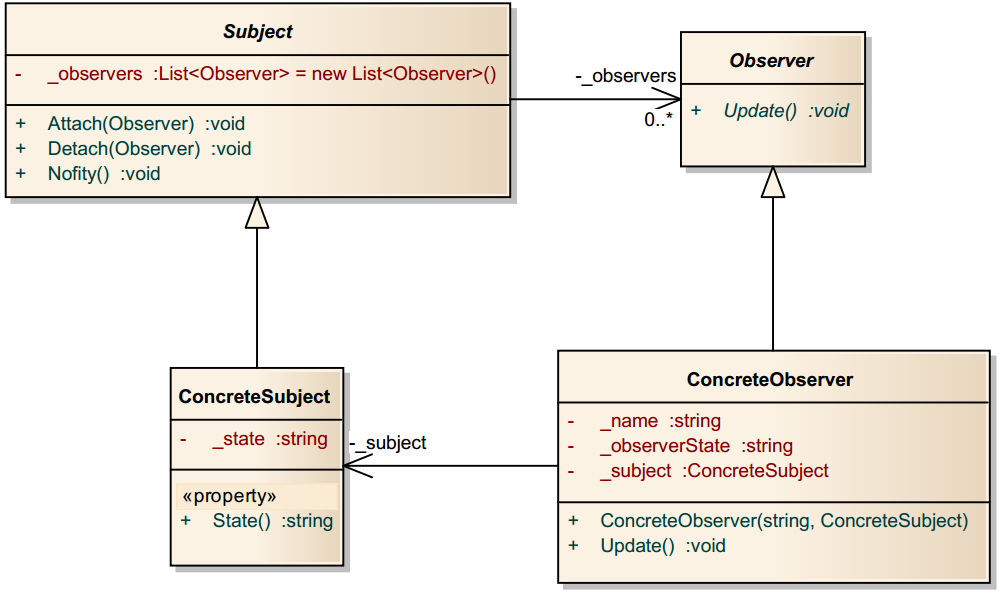
\includegraphics[width=\linewidth]{figs/observer_classdiagram}
	\caption[GoF Observer klassediagram]{Klassediagram som viser GoF Observers opbygning.}
	\label{fig:observer_classdiagram}
\end{figure}


\subsection{Sammenlign de forskellige varianter, af GoF Observer - hvilken vil du anvende hvornår?}

\subsection{Redegør for, hvordan anvendelsen af GoF Observer fremmer godt software design}

\subsection{Redegør for fordele og ulemper ved anvendelsen af GoF Observer}

\subsection{Redegør for, hvilke(t) SOLID-princip(per) du mener anvendelsen af GoF Observer undersøtter}

\begin{itemize}
	\item SRP.
	\item OCP.
	\item LSP.
	\item ISP.
	\item DIP.
\end{itemize}